\subsubsection{UC14 - Visualizzazione contenuto dizionario dati}\label{UC14}

\begin{figure}[H]
  \centering
  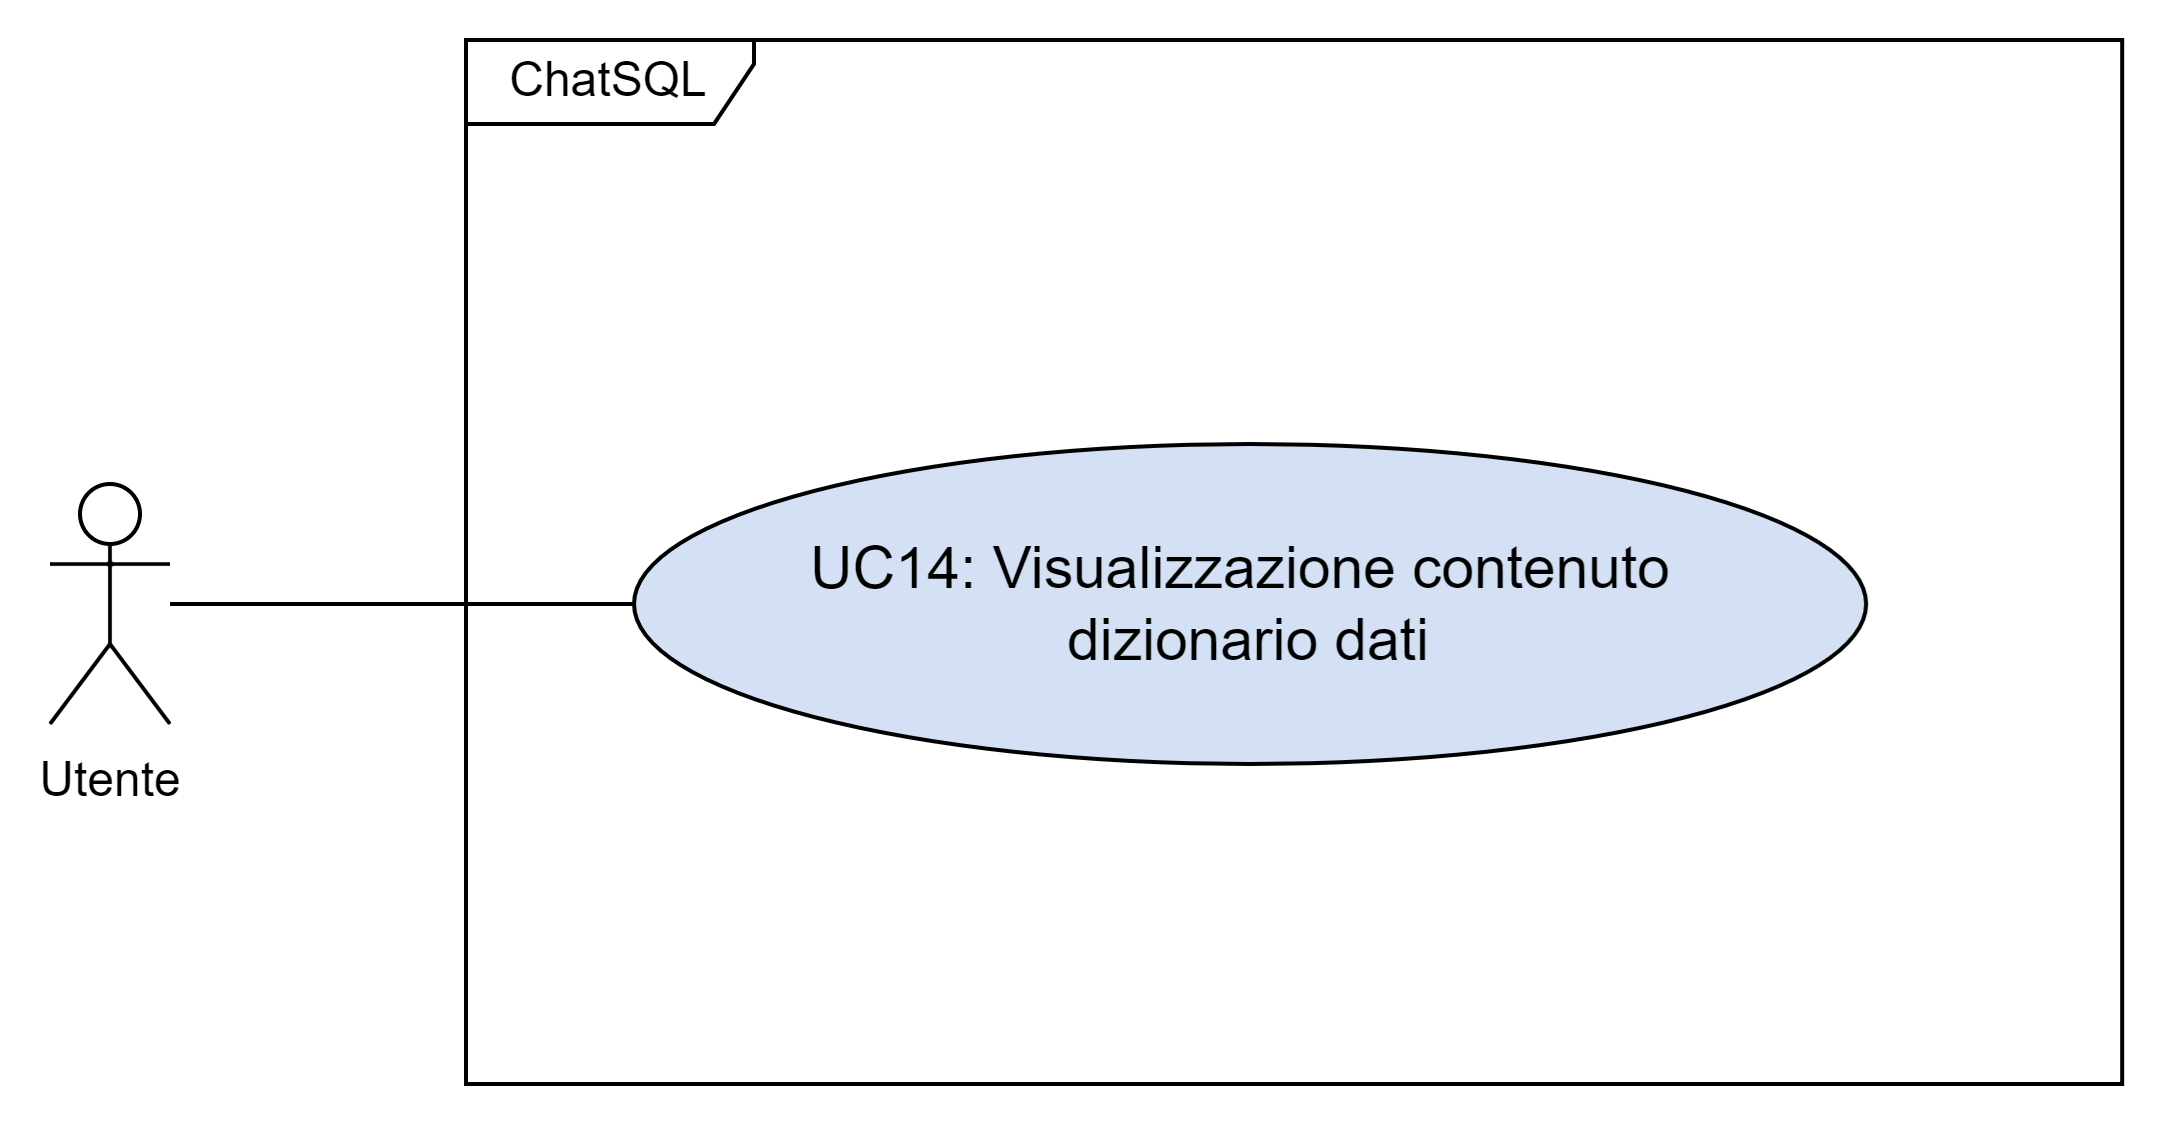
\includegraphics[width=0.90\textwidth]{assets/uc14.png}
  \caption{UC14}
\end{figure}

\paragraph*{Descrizione}
L'Utente visualizza il contenuto del \glossario{dizionario dati} selezionato. La visualizzazione del contenuto del dizionario può aiutare l'Utente a formulare correttamente la richiesta per il \glossario{modello}. Questa operazione equivale a visualizzare un'anteprima del dizionario dati.

\paragraph*{Attori principali}
Utente

\paragraph*{Precondizioni}
\begin{itemize}
  \item Il sistema è attivo e funzionante;
  \item L'Utente ha selezionato un \glossario{dizionario dati} (\hyperref[UC4]{UC4}).
\end{itemize}

\paragraph*{Postcondizioni}
\begin{itemize}
  \item Viene visualizzato il contenuto del dizionario scelto.
\end{itemize}

\paragraph*{Trigger}
L'Utente desidera visualizzare il contenuto di un \glossario{dizionario dati}.

\paragraph*{Scenario principale}
\begin{enumerate}
  \item Il sistema mostra il contenuto del dizionario in un formato comprensibile per l'Utente.
\end{enumerate}

\paragraph*{Sottocasi d'uso:}
\begin{itemize}
  \item \hyperref[UC14point1]{UC14.1}: Visualizzazione nome database;
  \item \hyperref[UC14point2]{UC14.2}: Visualizzazione descrizione database;
  \item \hyperref[UC14point3]{UC14.3}: Visualizzazione lista tabelle.
\end{itemize}

\begin{figure}[H]
  \centering
  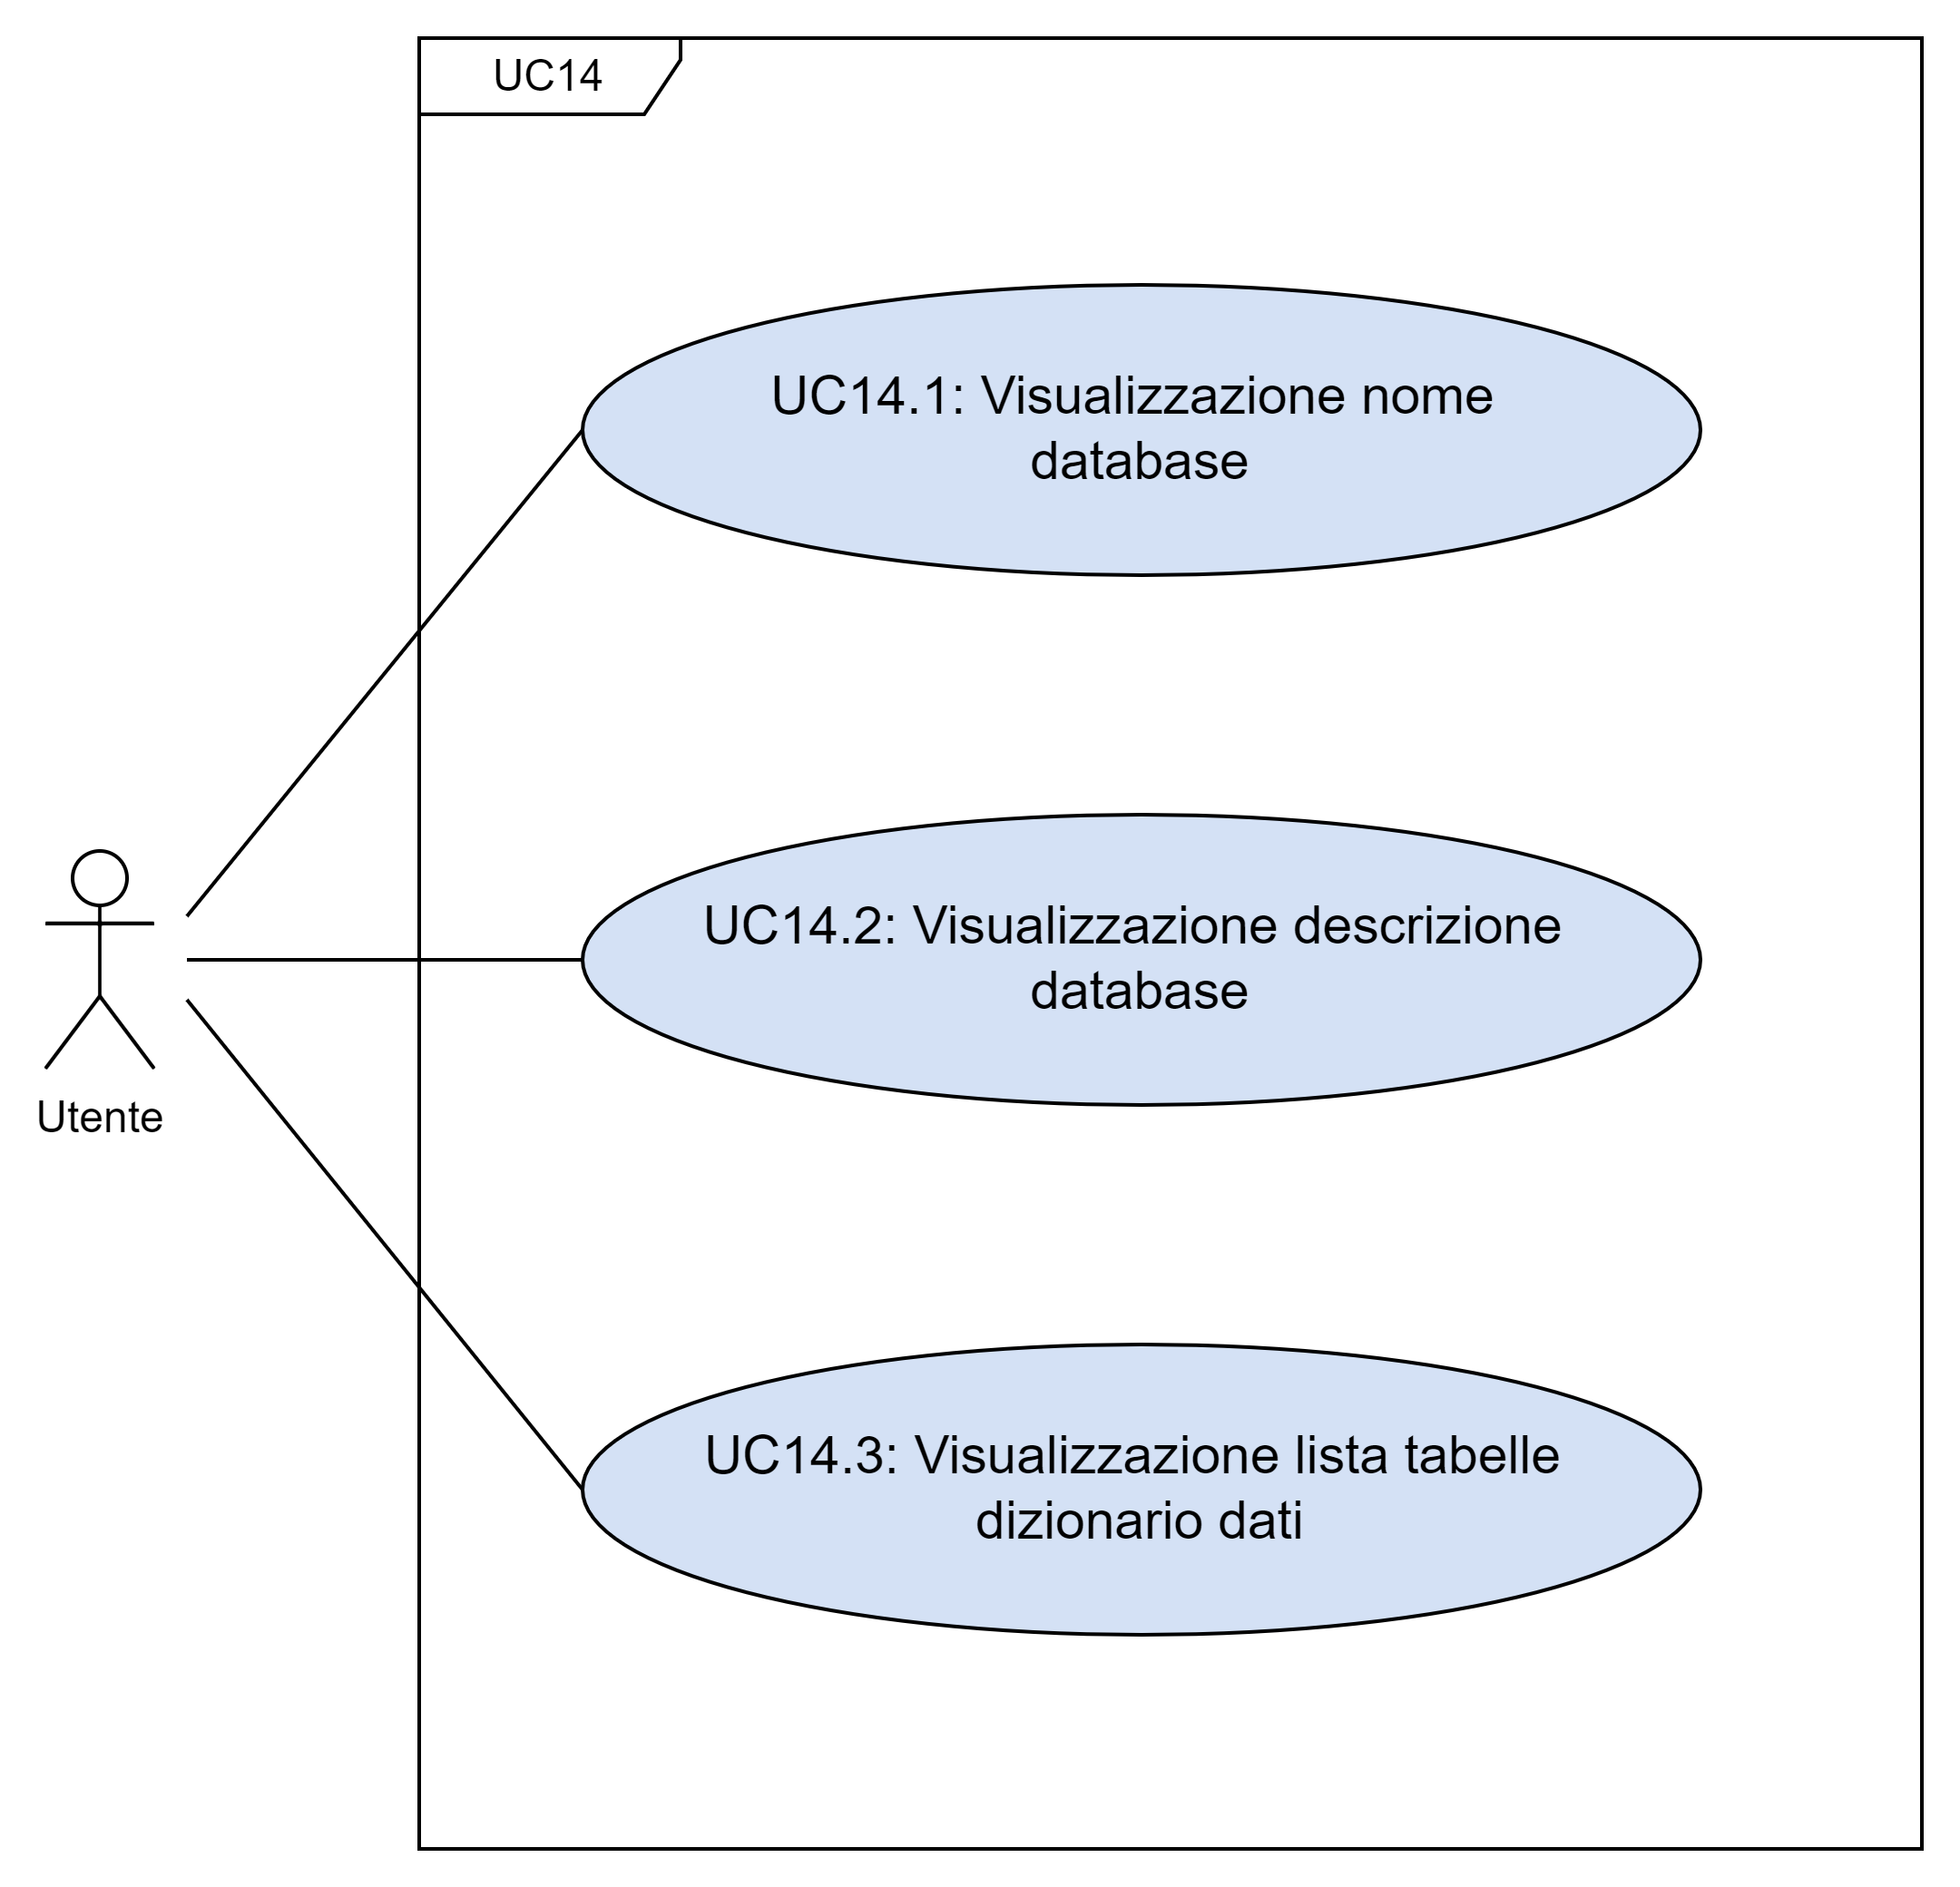
\includegraphics[width=0.90\textwidth]{assets/uc14_1.png}
  \caption{UC14 - Sottocasi d'uso}
\end{figure}

%%%%%%%%%%%%%%%%%%%%%%%%%%%%%%%%%%%%%%%%%%%%%%%%%%%%%%%%%%%%%%%%%%%%%%%%%%%%%%

\subsubsection{UC14.1 - Visualizzazione nome database}\label{UC14point1}
\paragraph*{Descrizione}
L'Utente visualizza il nome del database descritto nel \glossario{dizionario dati}.

\paragraph*{Attori principali}
Utente

\paragraph*{Precondizioni}
\begin{itemize}
  \item L'Utente ha selezionato un \glossario{dizionario dati} (\hyperref[UC4]{UC4}).
\end{itemize}

\paragraph*{Postcondizioni}
\begin{itemize}
  \item Il nome del database viene visualizzato correttamente.
\end{itemize}

\paragraph*{Trigger}
L'Utente desidera visualizzare il nome del database.

\paragraph*{Scenario principale}
\begin{enumerate}
  \item L'Utente visualizza il nome del database.
\end{enumerate}

%%%%%%%%%%%%%%%%%%%%%%%%%%%%%%%%%%%%%%%%%%%%%%%%%%%%%%%%%%%%%%%%%%%%%%%%%%%%%%

\subsubsection{UC14.2 - Visualizzazione descrizione database}\label{UC14point2}
\paragraph*{Descrizione}
L'Utente visualizza la descrizione del database riportato nel \glossario{dizionario dati}.

\paragraph*{Attori principali}
Utente

\paragraph*{Precondizioni}
\begin{itemize}
  \item L'Utente ha selezionato un \glossario{dizionario dati} (\hyperref[UC4]{UC4}).
\end{itemize}

\paragraph*{Postcondizioni}
\begin{itemize}
  \item La descrizione del database viene visualizzata correttamente.
\end{itemize}

\paragraph*{Trigger}
L'Utente desidera visualizzare la descrizione del database.

\paragraph*{Scenario principale}
\begin{enumerate}
  \item L'Utente visualizza la descrizione del database.
\end{enumerate}

%%%%%%%%%%%%%%%%%%%%%%%%%%%%%%%%%%%%%%%%%%%%%%%%%%%%%%%%%%%%%%%%%%%%%%%%%%%%%%

\subsubsection{UC14.3 - Visualizzazione lista tabelle dizionario dati}\label{UC14point3}
\paragraph*{Descrizione}
L'Utente visualizza la lista delle tabelle descritte nel \glossario{dizionario dati}.

\paragraph*{Attori principali}
Utente

\paragraph*{Precondizioni}
\begin{itemize}
  \item L'Utente ha selezionato un \glossario{dizionario dati} (\hyperref[UC4]{UC4}).
\end{itemize}

\paragraph*{Postcondizioni}
\begin{itemize}
  \item La lista delle tabelle viene visualizzata correttamente.
\end{itemize}

\paragraph*{Trigger}
L'Utente desidera visualizzare la lista delle tabelle.

\paragraph*{Scenario principale}
\begin{enumerate}
  \item L'Utente visualizza la lista delle tabelle.
\end{enumerate}

\paragraph*{Sottocasi d'uso:}
\begin{itemize}
  \item \hyperref[UC14point3point1]{UC14.3.1}: Visualizzazione singola tabella.
\end{itemize}

%%%%%%%%%%%%%%%%%%%%%%%%%%%%%%%%%%%%%%%%%%%%%%%%%%%%%%%%%%%%%%%%%%%%%%%%%%%%%%

\subsubsection{UC14.3.1 - Visualizzazione singola tabella dizionario dati}\label{UC14point3point1}

\begin{figure}[H]
  \centering
  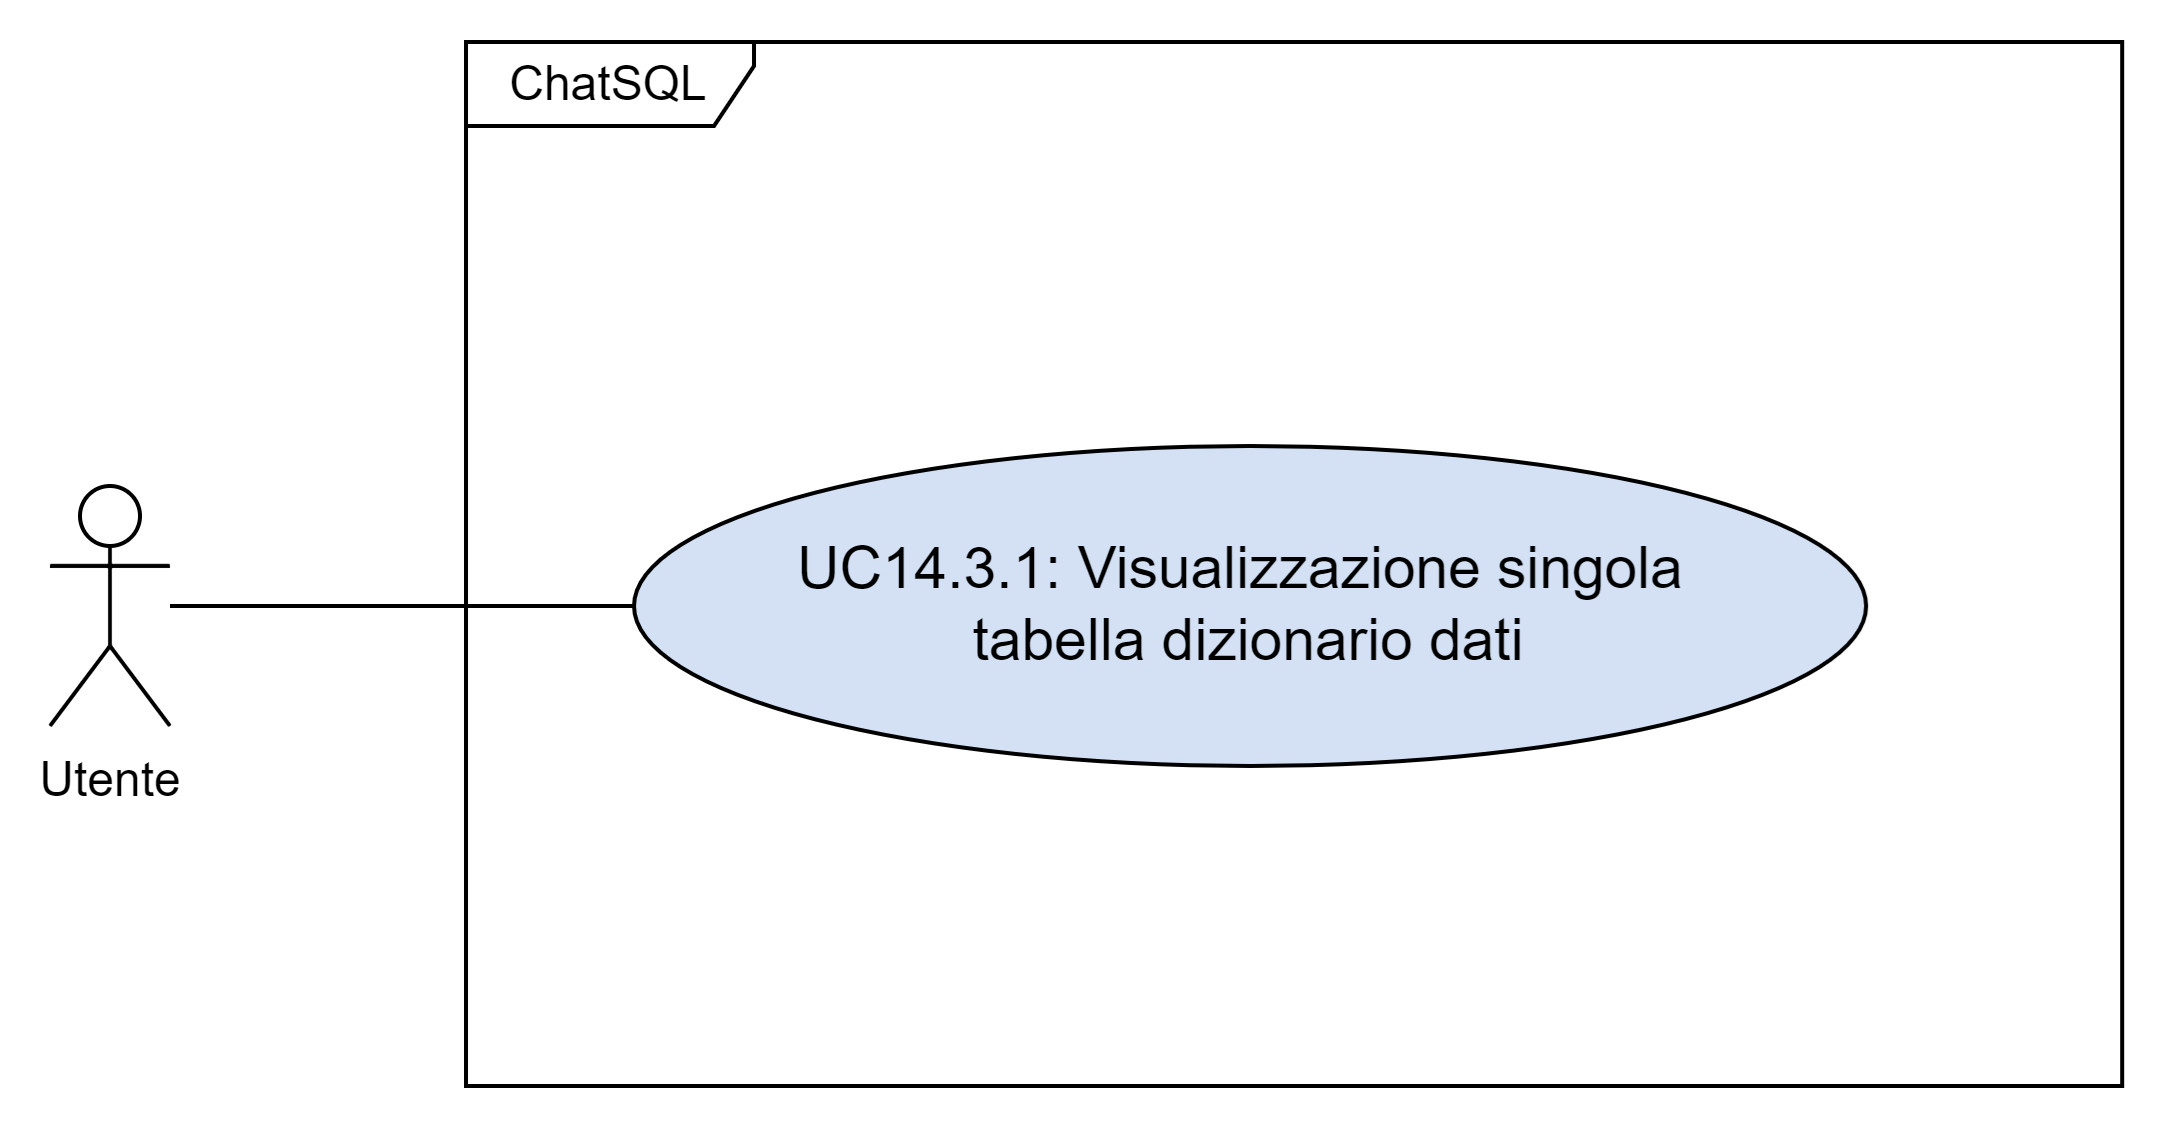
\includegraphics[width=0.90\textwidth]{assets/uc14_3_1.png}
  \caption{UC14.3.1}
\end{figure}

\paragraph*{Descrizione}
L'Utente visualizza una tabella tra quelle descritte nel \glossario{dizionario dati}.

\paragraph*{Attori principali}
Utente

\paragraph*{Precondizioni}
\begin{itemize}
  \item L'Utente ha selezionato un \glossario{dizionario dati} (\hyperref[UC4]{UC4});
  \item L'Utente ha visualizzato la lista delle tabelle (\hyperref[UC14point3]{UC14.3}).
\end{itemize}

\paragraph*{Postcondizioni}
\begin{itemize}
  \item La tabella viene visualizzata correttamente.
\end{itemize}

\paragraph*{Trigger}
L'Utente desidera visualizzare una tabella con le sue informazioni.

\paragraph*{Scenario principale}
\begin{enumerate}
  \item L'Utente visualizza una singola tabella in lista.
\end{enumerate}

\paragraph*{Sottocasi d'uso:}
\begin{itemize}
  \item \hyperref[UC14point3point1point1]{UC14.3.1.1}: Visualizzazione nome tabella;
  \item \hyperref[UC14point3point1point2]{UC14.3.1.2}: Visualizzazione descrizione tabella.
\end{itemize}

\begin{figure}[H]
  \centering
  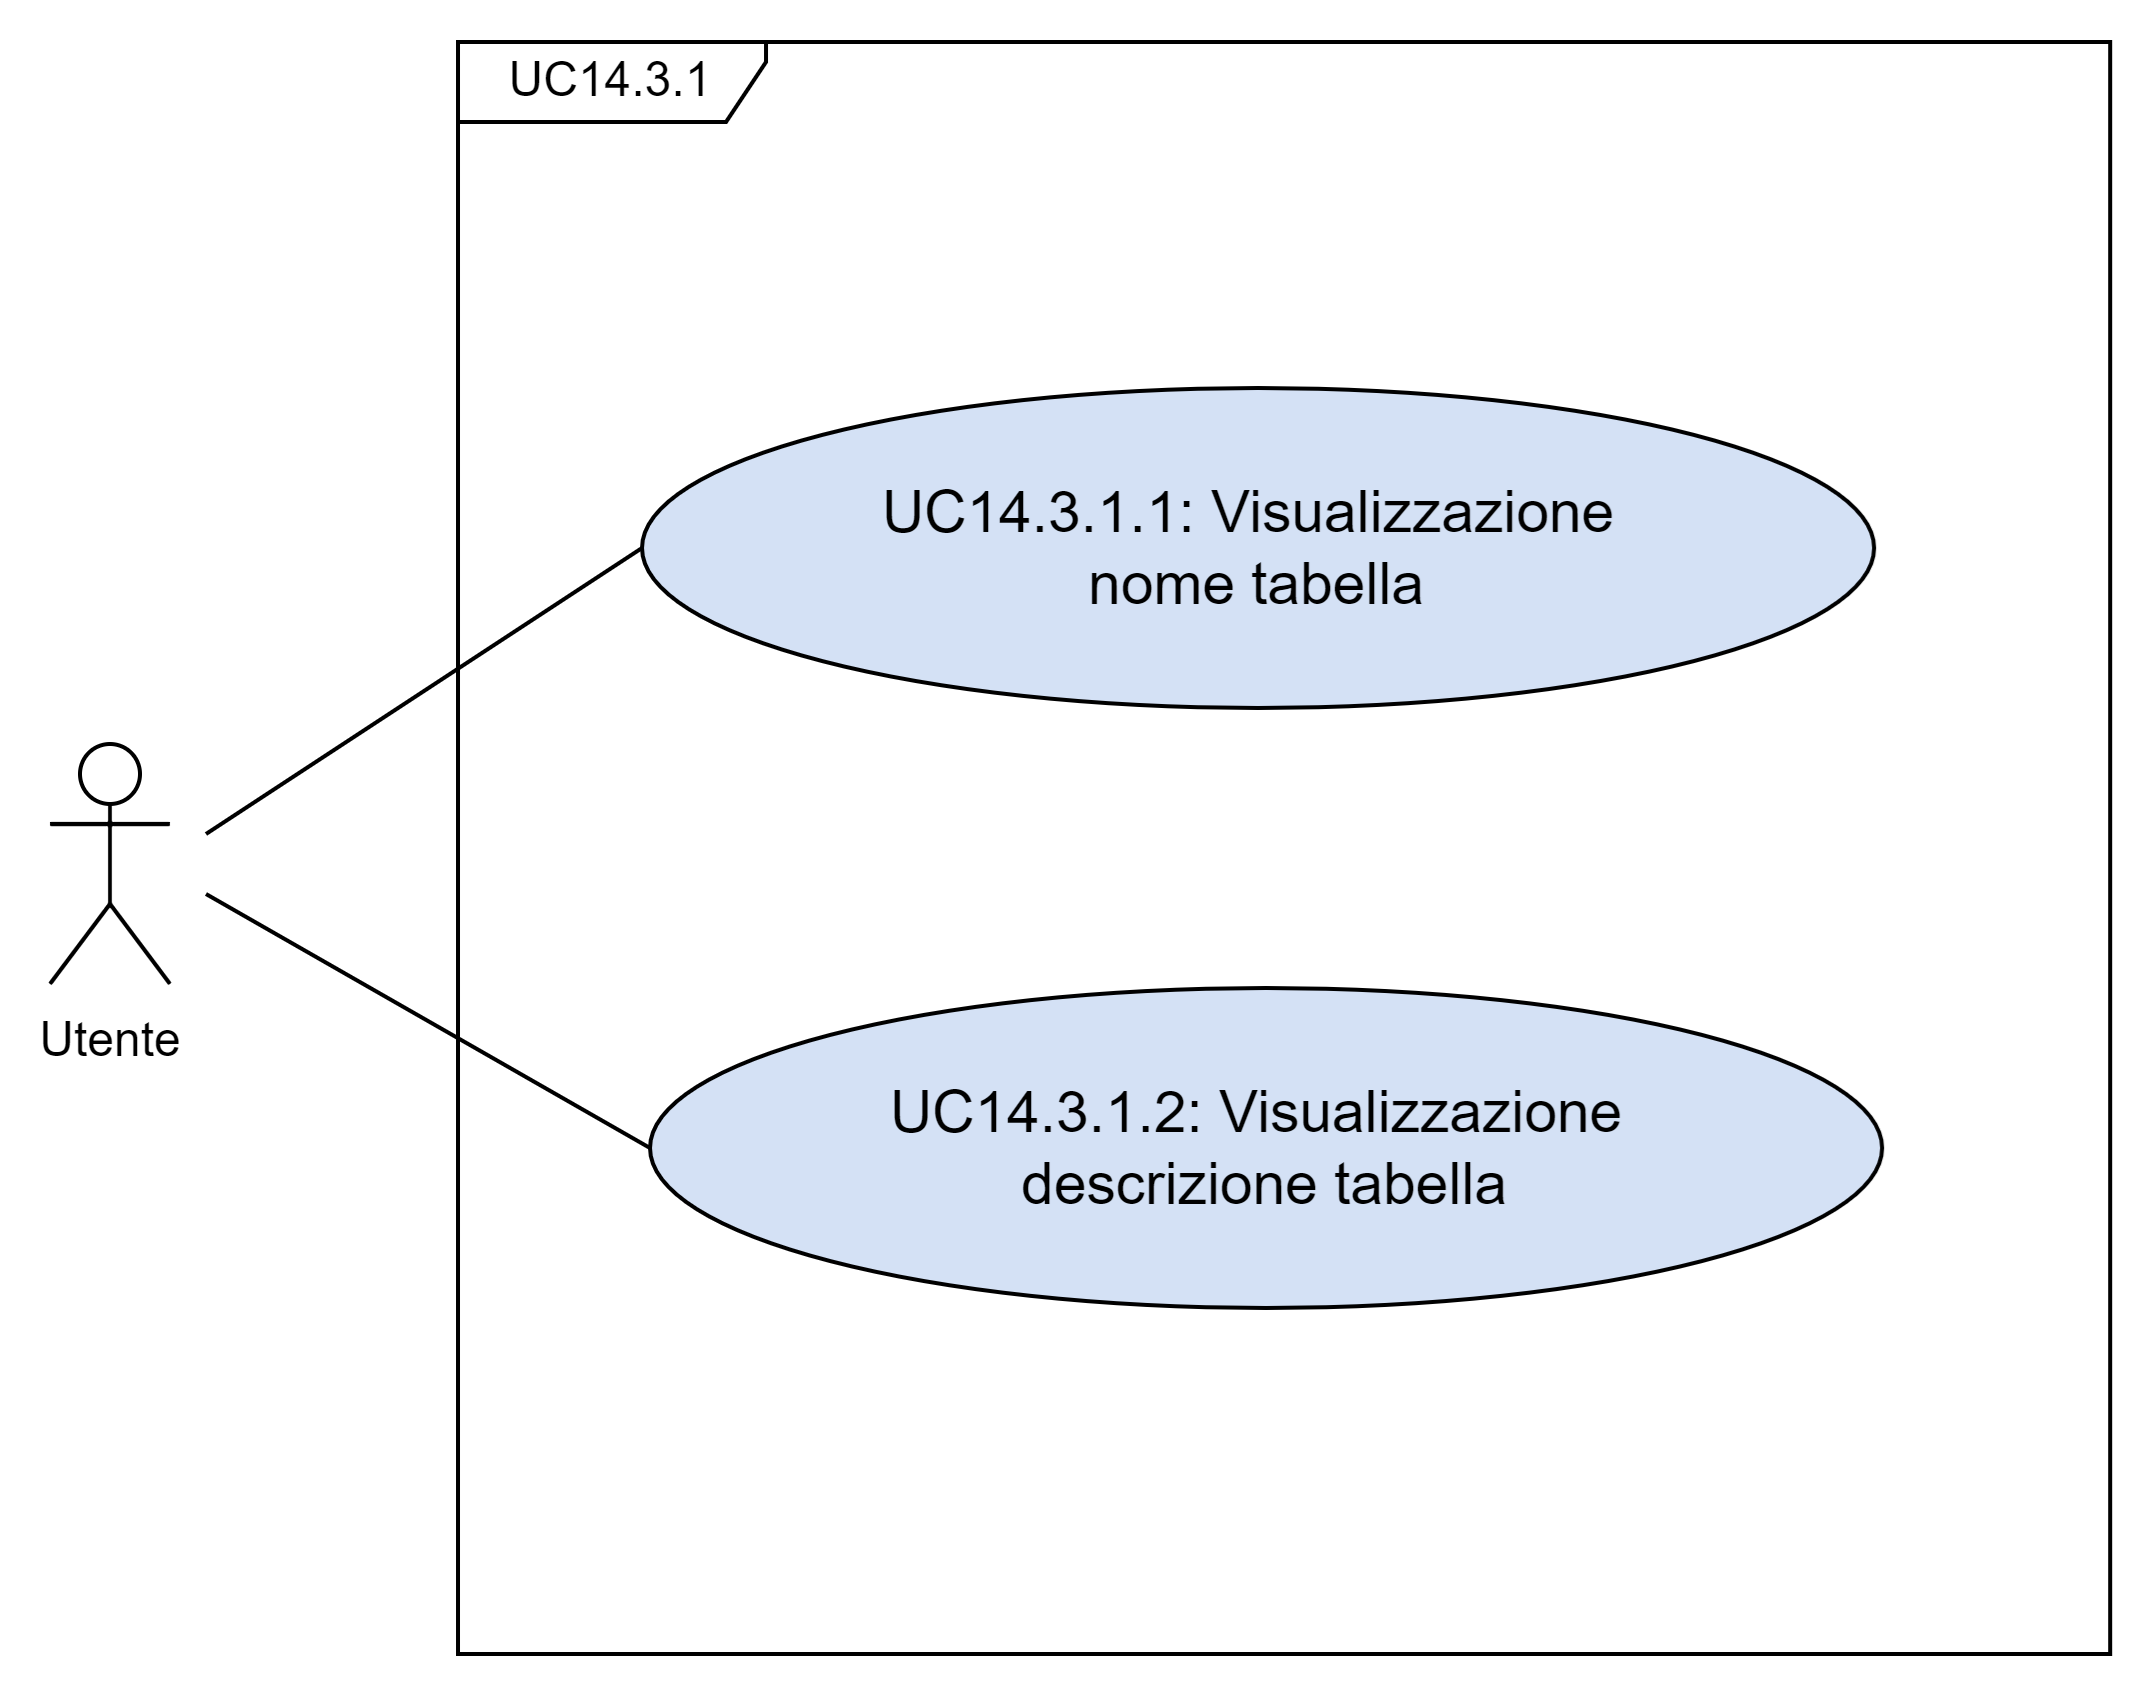
\includegraphics[width=0.90\textwidth]{assets/uc14_3_1_1.png}
  \caption{UC14.3.1 - Sottocasi d'uso}
\end{figure}

%%%%%%%%%%%%%%%%%%%%%%%%%%%%%%%%%%%%%%%%%%%%%%%%%%%%%%%%%%%%%%%%%%%%%%%%%%%%%%

\subsubsection{UC14.3.1.1 - Visualizzazione nome tabella}\label{UC14point3point1point1}
\paragraph*{Descrizione}
L'Utente visualizza il nome di una tabella.

\paragraph*{Attori principali}
Utente

\paragraph*{Precondizioni}
\begin{itemize}
  \item L'Utente ha selezionato un \glossario{dizionario dati} (\hyperref[UC4]{UC4});
  \item L'Utente ha visualizzato la lista delle tabelle (\hyperref[UC14point3]{UC14.3});
  \item L'Utente ha visualizzato una singola tabella in lista (\hyperref[UC14point3point1]{UC14.3.1}).
\end{itemize}

\paragraph*{Postcondizioni}
\begin{itemize}
  \item Il nome della tabella viene visualizzato correttamente.
\end{itemize}

\paragraph*{Trigger}
L'Utente desidera visualizzare il nome di una tabella.

\paragraph*{Scenario principale}
\begin{enumerate}
  \item L'Utente visualizza il nome di una tabella.
\end{enumerate}

%%%%%%%%%%%%%%%%%%%%%%%%%%%%%%%%%%%%%%%%%%%%%%%%%%%%%%%%%%%%%%%%%%%%%%%%%%%%%%

\subsubsection{UC14.3.1.2 - Visualizzazione descrizione tabella}\label{UC14point3point1point2}
\paragraph*{Descrizione}
L'Utente visualizza la descrizione di una tabella.

\paragraph*{Attori principali}
Utente

\paragraph*{Precondizioni}
\begin{itemize}
  \item L'Utente ha selezionato un \glossario{dizionario dati} (\hyperref[UC4]{UC4});
  \item L'Utente ha visualizzato la lista delle tabelle (\hyperref[UC14point3]{UC14.3});
  \item L'Utente ha visualizzato una singola tabella in lista (\hyperref[UC14point3point1]{UC14.3.1}).
\end{itemize}

\paragraph*{Postcondizioni}
\begin{itemize}
  \item La descrizione della tabella viene visualizzata correttamente.
\end{itemize}

\paragraph*{Trigger}
L'Utente desidera visualizzare la descrizione di una tabella.

\paragraph*{Scenario principale}
\begin{enumerate}
  \item L'Utente visualizza la descrizione di una tabella.
\end{enumerate}